% Options for packages loaded elsewhere
\PassOptionsToPackage{unicode}{hyperref}
\PassOptionsToPackage{hyphens}{url}
\documentclass[
  ignorenonframetext,
]{beamer}
\newif\ifbibliography
\usepackage{pgfpages}
\setbeamertemplate{caption}[numbered]
\setbeamertemplate{caption label separator}{: }
\setbeamercolor{caption name}{fg=normal text.fg}
\beamertemplatenavigationsymbolsempty
% remove section numbering
\setbeamertemplate{part page}{
  \centering
  \begin{beamercolorbox}[sep=16pt,center]{part title}
    \usebeamerfont{part title}\insertpart\par
  \end{beamercolorbox}
}
\setbeamertemplate{section page}{
  \centering
  \begin{beamercolorbox}[sep=12pt,center]{section title}
    \usebeamerfont{section title}\insertsection\par
  \end{beamercolorbox}
}
\setbeamertemplate{subsection page}{
  \centering
  \begin{beamercolorbox}[sep=8pt,center]{subsection title}
    \usebeamerfont{subsection title}\insertsubsection\par
  \end{beamercolorbox}
}
% Prevent slide breaks in the middle of a paragraph
\widowpenalties 1 10000
\raggedbottom
\AtBeginPart{
  \frame{\partpage}
}
\AtBeginSection{
  \ifbibliography
  \else
    \frame{\sectionpage}
  \fi
}
\AtBeginSubsection{
  \frame{\subsectionpage}
}
\usepackage{iftex}
\ifPDFTeX
  \usepackage[T1]{fontenc}
  \usepackage[utf8]{inputenc}
  \usepackage{textcomp} % provide euro and other symbols
\else % if luatex or xetex
  \usepackage{unicode-math} % this also loads fontspec
  \defaultfontfeatures{Scale=MatchLowercase}
  \defaultfontfeatures[\rmfamily]{Ligatures=TeX,Scale=1}
\fi
\usepackage{lmodern}
\ifPDFTeX\else
  % xetex/luatex font selection
\fi
% Use upquote if available, for straight quotes in verbatim environments
\IfFileExists{upquote.sty}{\usepackage{upquote}}{}
\IfFileExists{microtype.sty}{% use microtype if available
  \usepackage[]{microtype}
  \UseMicrotypeSet[protrusion]{basicmath} % disable protrusion for tt fonts
}{}
\makeatletter
\@ifundefined{KOMAClassName}{% if non-KOMA class
  \IfFileExists{parskip.sty}{%
    \usepackage{parskip}
  }{% else
    \setlength{\parindent}{0pt}
    \setlength{\parskip}{6pt plus 2pt minus 1pt}}
}{% if KOMA class
  \KOMAoptions{parskip=half}}
\makeatother
\usepackage{longtable,booktabs,array}
\usepackage{caption}
\captionsetup[table]{skip=6pt}
\newcounter{none} % for unnumbered tables
\usepackage{calc} % for calculating minipage widths
\usepackage{caption}
% Make caption package work with longtable
\makeatletter
\def\fnum@table{\tablename~\thetable}
\makeatother
\usepackage{graphicx}
\makeatletter
\newsavebox\pandoc@box
\newcommand*\pandocbounded[1]{% scales image to fit in text height/width
  \sbox\pandoc@box{#1}%
  \Gscale@div\@tempa{\textheight}{\dimexpr\ht\pandoc@box+\dp\pandoc@box\relax}%
  \Gscale@div\@tempb{\linewidth}{\wd\pandoc@box}%
  \ifdim\@tempb\p@<\@tempa\p@\let\@tempa\@tempb\fi% select the smaller of both
  \ifdim\@tempa\p@<\p@\scalebox{\@tempa}{\usebox\pandoc@box}%
  \else\usebox{\pandoc@box}%
  \fi%
}
% Set default figure placement to htbp
\def\fps@figure{htbp}
\makeatother
\setlength{\emergencystretch}{3em} % prevent overfull lines
\providecommand{\tightlist}{%
  \setlength{\itemsep}{0pt}\setlength{\parskip}{0pt}}
% Manuscript macro/package fallbacks (newcommand -> providecommand).
% Core mathematical packages
\usepackage{amsmath,amssymb,amsthm}
\usepackage{mathtools}
% Keep long deployment prose and references within the text block.
% Algorithm formatting
% Tables
\usepackage{booktabs}
\usepackage{multirow}
% Graphics and floats
% Typography and layout
% Page layout (slightly smaller margins for academic journal style)
% Running headers/footers
% Caption formatting
% Colored boxes for callouts
% Cross-referencing with smart naming
% Hyperlink styling
% Configure cleveref for custom environments
% Theorem environments with consistent numbering
% Code listings and raw implementation examples in the manuscript
\usepackage{listings}
\lstset{basicstyle=\ttfamily\small,breaklines=true,columns=fullflexible}
% Math operators
\DeclareMathOperator*{\argmax}{arg\,max}
\DeclareMathOperator*{\argmin}{arg\,min}
\DeclareMathOperator{\sign}{sign}
\DeclareMathOperator{\KL}{KL}
\DeclareMathOperator{\Tr}{Tr}
% Custom commands for notation consistency
\providecommand{\calA}{\mathcal{A}}
\providecommand{\calB}{\mathcal{B}}
\providecommand{\calC}{\mathcal{C}}
\providecommand{\calD}{\mathcal{D}}
\providecommand{\calF}{\mathcal{F}}
\providecommand{\calG}{\mathcal{G}}
\providecommand{\calH}{\mathcal{H}}
\providecommand{\calI}{\mathcal{I}}
\providecommand{\calM}{\mathcal{M}}
\providecommand{\calO}{\mathcal{O}}
\providecommand{\calP}{\mathcal{P}}
\providecommand{\calS}{\mathcal{S}}
\providecommand{\calT}{\mathcal{T}}
\providecommand{\calW}{\mathcal{W}}
% Note: \Phi is a standard LaTeX command, do not redefine
% Trust notation
\providecommand{\trust}[2]{\mathcal{T}_{#1 \to #2}}
\providecommand{\trustt}[3]{\mathcal{T}_{#1 \to #2}^{#3}}
% Belief notation
\providecommand{\belief}[2]{\mathcal{B}_{#1}(#2)}
\providecommand{\belieft}[3]{\mathcal{B}_{#1}^{#2}(#3)}
% Cognitive state
\providecommand{\cogstate}[1]{\sigma_{#1}}
% Attack notation
\providecommand{\attack}[1]{\mathcal{A}_{#1}}
\providecommand{\adversary}[1]{\Omega_{#1}}
% Defense notation
\providecommand{\firewall}{\mathcal{F}}
\providecommand{\sandbox}{\mathcal{S}_{box}}
% Probability and expectation
\providecommand{\E}{\mathbb{E}}
\providecommand{\Prob}{\mathbb{P}}
\providecommand{\indicator}{\mathbb{1}}
% QED symbol
\providecommand{\qedsymbol}{$\blacksquare$}
% Front matter opens on the cover/title page (no list of figures/tables precedes it).

% Slide layout defaults for warning-clean scientific decks.
\usepackage{etoolbox}
\IfFileExists{xurl.sty}{\usepackage{xurl}}{}
\IfFileExists{seqsplit.sty}{\usepackage{seqsplit}}{\newcommand{\seqsplit}[1]{#1}}
\protected\def\breakseq#1{\seqsplit{#1}}
\protected\def\breaktt#1{\begingroup\ttfamily\seqsplit{#1}\endgroup}
\setlength{\emergencystretch}{6em}
\tolerance=5000
\hbadness=10000
\hfuzz=1pt
\setlength{\tabcolsep}{2pt}
\AtBeginEnvironment{longtable}{\tiny\renewcommand{\arraystretch}{0.86}\setlength{\tabcolsep}{1pt}}
\AtBeginEnvironment{tabular}{\tiny\renewcommand{\arraystretch}{0.86}\setlength{\tabcolsep}{1pt}}
\AtBeginEnvironment{equation}{\tiny}
\AtBeginEnvironment{equation*}{\tiny}
\AtBeginEnvironment{align}{\tiny}
\AtBeginEnvironment{align*}{\tiny}
\AtBeginEnvironment{itemize}{\footnotesize}
\AtBeginEnvironment{enumerate}{\footnotesize}
\AtBeginEnvironment{description}{\footnotesize}
\setbeamerfont{caption}{size=\tiny}
\setbeamerfont{caption name}{size=\tiny}
\setbeamerfont{normal text}{size=\small}
\setbeamerfont{frametitle}{size=\small}
\setbeamerfont{section title}{size=\footnotesize}
\setbeamerfont{subsection title}{size=\footnotesize}
\setbeamertemplate{section page}{%
  \centering
  \begin{beamercolorbox}[sep=12pt,center,wd=\paperwidth]{section title}
    \parbox{0.86\paperwidth}{\centering\usebeamerfont{section title}\insertsection\par}
  \end{beamercolorbox}
}
\setbeamertemplate{subsection page}{%
  \centering
  \begin{beamercolorbox}[sep=8pt,center,wd=\paperwidth]{subsection title}
    \parbox{0.86\paperwidth}{\centering\usebeamerfont{subsection title}\insertsubsection\par}
  \end{beamercolorbox}
}
\setlength{\abovecaptionskip}{2pt}
\setlength{\belowcaptionskip}{0pt}

% Natbib and cross-reference fallbacks — slides don't load natbib
% or cleveref, but combined-PDF manuscript prose may emit these
% commands. The fallback renders citations as a bracketed key list
% and cross-references as detokenized labels so slides don't fail on
% undefined control sequences or raw underscores. \providecommand is
% a no-op if packages load later.
\providecommand{\citep}[1]{[#1]}
\providecommand{\citet}[1]{#1}
\providecommand{\citealp}[1]{#1}
\providecommand{\citeauthor}[1]{#1}
\providecommand{\citeyear}[1]{#1}
\providecommand{\cref}[1]{\texttt{\detokenize{#1}}}
\providecommand{\Cref}[1]{\texttt{\detokenize{#1}}}
\providecommand{\crefrange}[2]{\texttt{\detokenize{#1}}--\texttt{\detokenize{#2}}}
\providecommand{\Crefrange}[2]{\texttt{\detokenize{#1}}--\texttt{\detokenize{#2}}}
\providecommand{\paragraph}[1]{\textbf{#1}\ }

\newtheorem{proposition}{Proposition}
\newtheorem{hypothesis}{Hypothesis}
\newtheorem{remark}[theorem]{Remark}
\newtheorem{axiom}{Axiom}
\newtheorem{property}{Property}
\usepackage{bookmark}
\IfFileExists{xurl.sty}{\usepackage{xurl}}{} % add URL line breaks if available
\urlstyle{same}
% fallback for those not using the hyperref driver hyperxmp:
\makeatletter
\@ifundefined{xmpquote}{\newcommand{\xmpquote}[1]{#1}}{}
\makeatother
\hypersetup{
  hidelinks,
  pdfcreator={LaTeX via pandoc}}

\author{\texorpdfstring{}{}}
\date{}

\begin{document}

\section{Deployment Profiles: Evaluated Configurations from Part
2}\label{sec:deployment}

\begin{frame}[allowframebreaks]{Deployment Profiles: Evaluated
Configurations from Part 2}
\begin{figure}
\centering
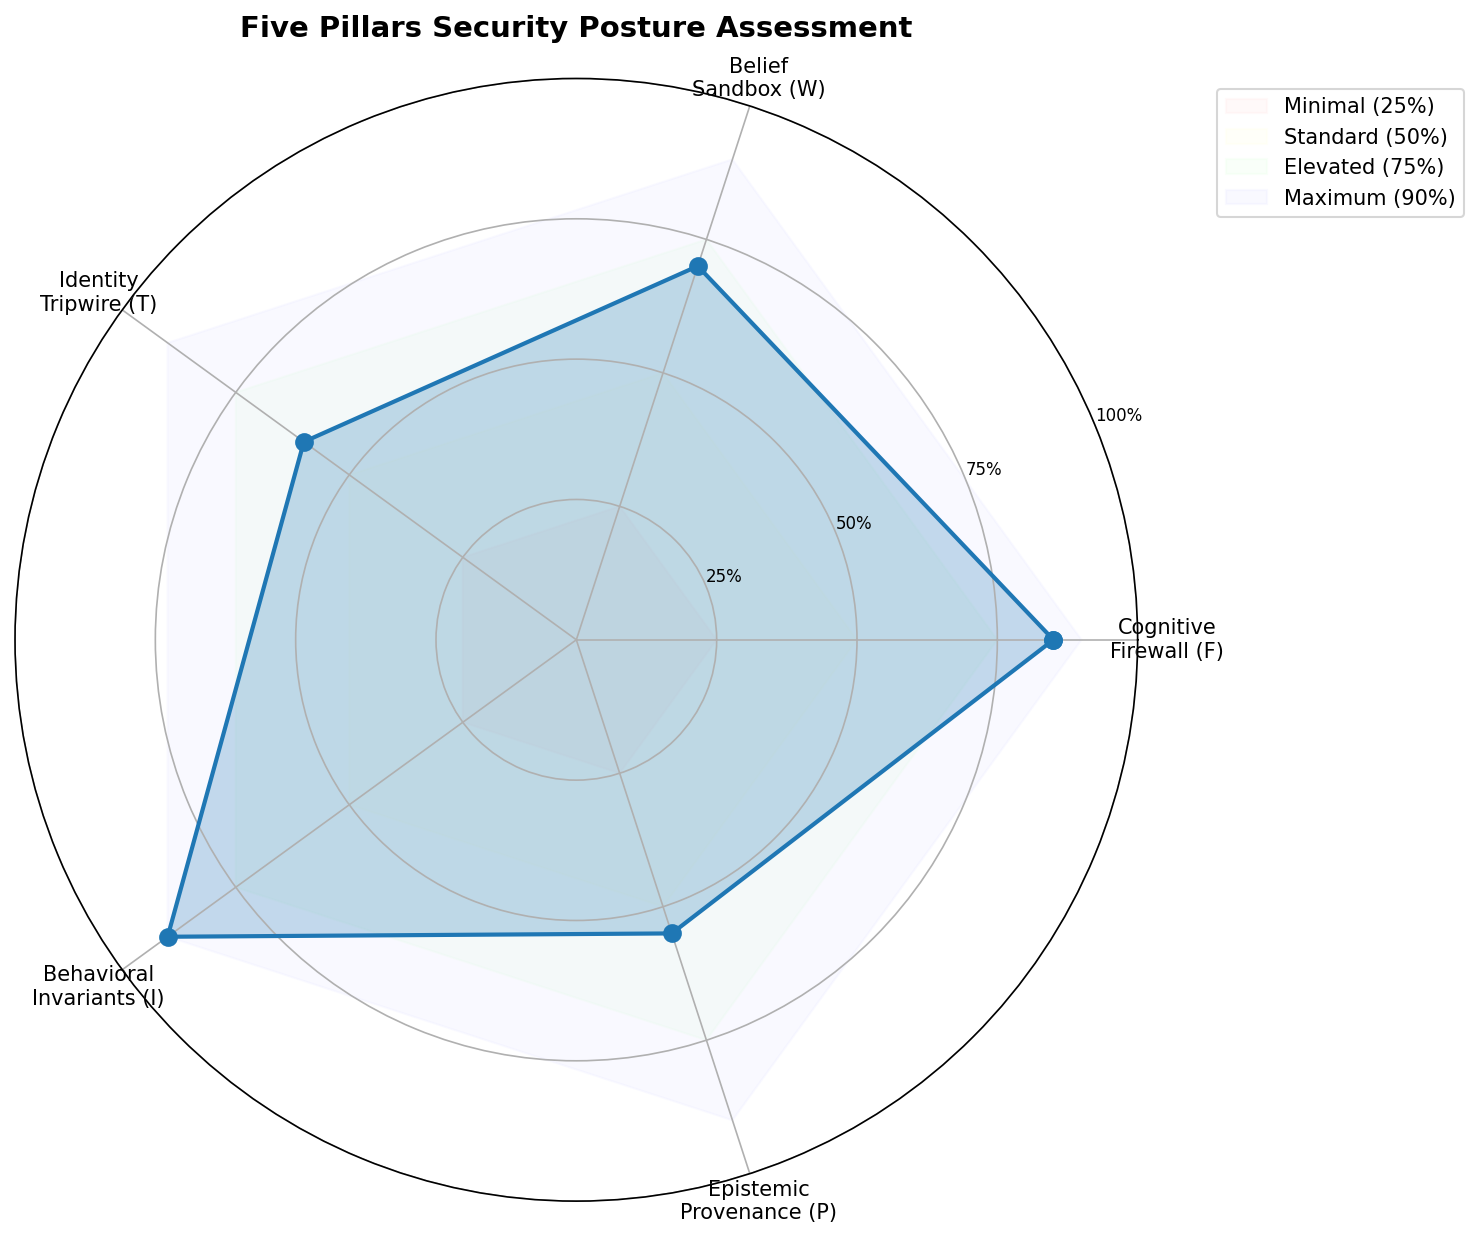
\includegraphics[width=0.8\linewidth,height=0.40\textheight,keepaspectratio,alt={Five-Pillar operator posture assessment radar (Cognitive Firewall, Belief Sandbox, Identity Tripwire, Behavioral Invariants, Provenance), color-coded against readiness thresholds.}]{../figures/posture_radar.png}
\caption{Five-Pillar operator posture assessment radar (Cognitive
Firewall, Belief Sandbox, Identity Tripwire, Behavioral Invariants,
Provenance), color-coded against readiness
thresholds.}\label{fig:posture-radar}
\end{figure}

\begin{figure}
\centering
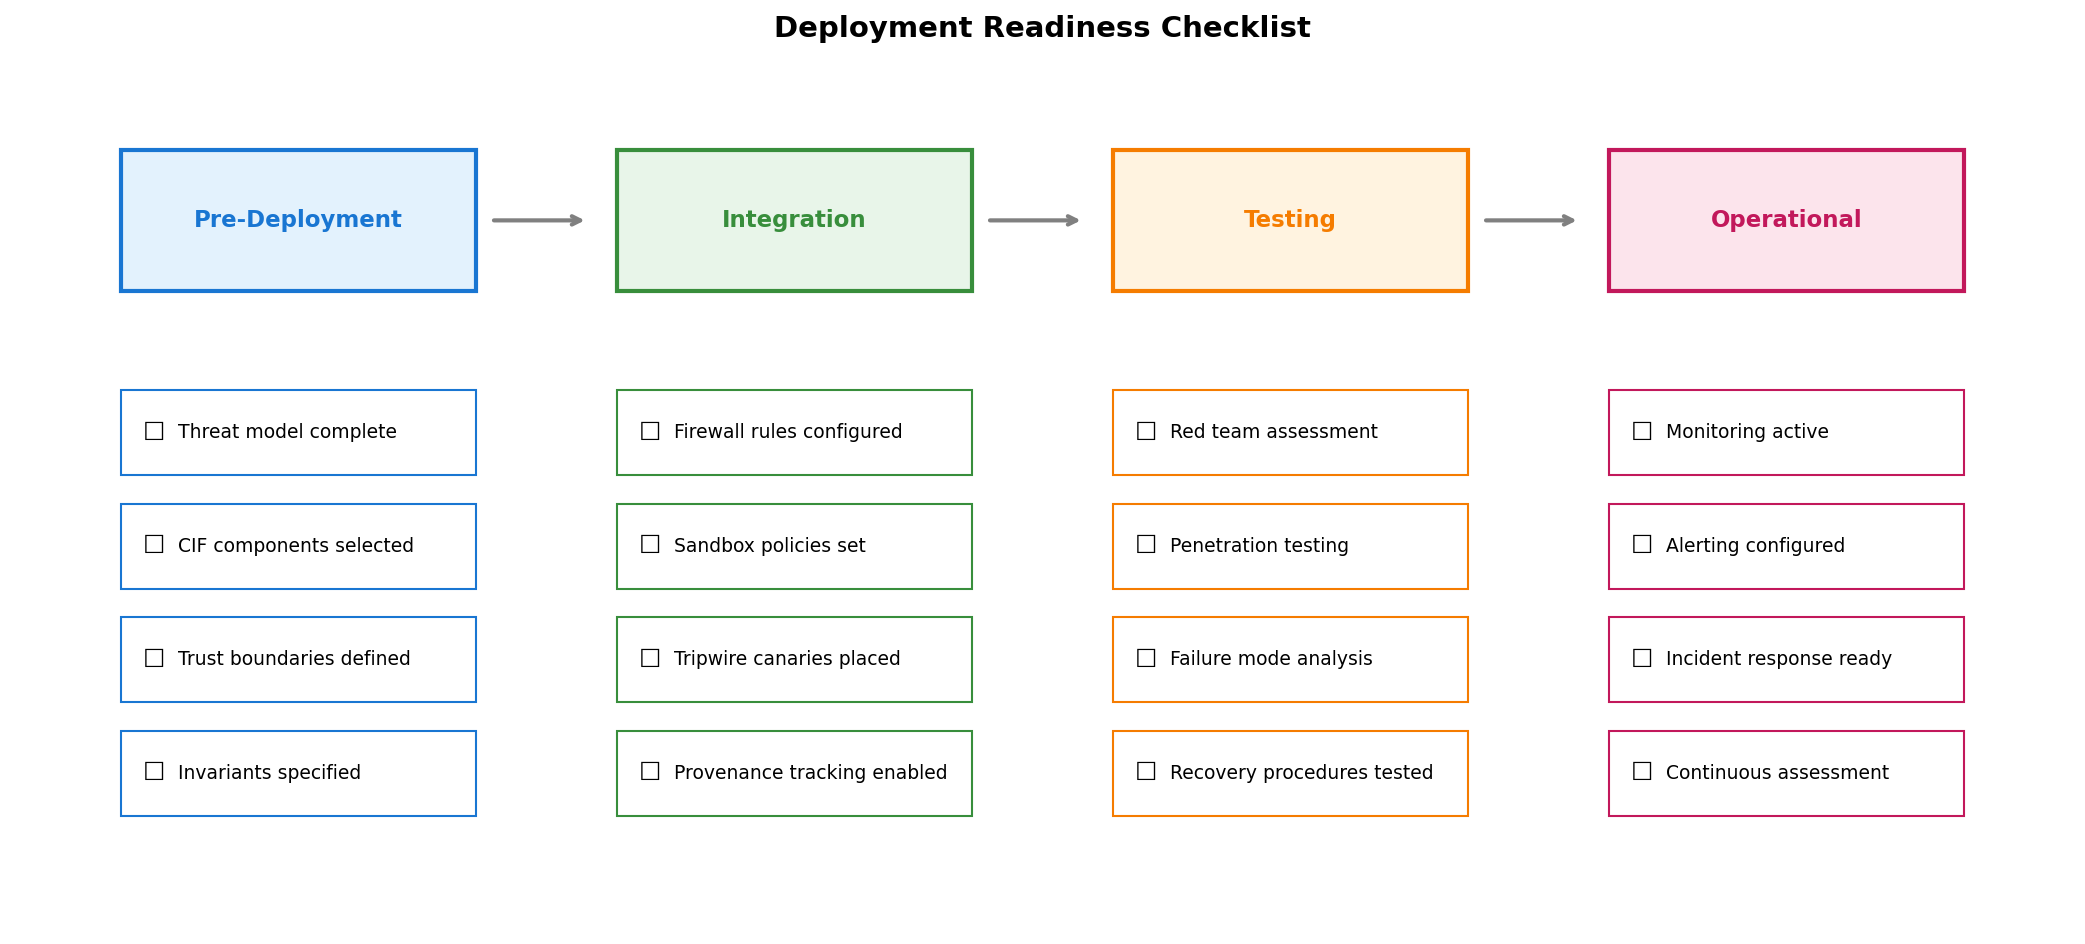
\includegraphics[width=0.85\linewidth,height=0.40\textheight,keepaspectratio,alt={Pre-deployment \textbackslash rightarrow Integration \textbackslash rightarrow Testing \textbackslash rightarrow Operational checklist flowchart mapping CIF enforcement points to deployment phases.}]{../figures/checklist_flowchart.png}
\caption{Pre-deployment \(\rightarrow\) Integration \(\rightarrow\)
Testing \(\rightarrow\) Operational checklist flowchart mapping CIF
enforcement points to deployment phases.}\label{fig:checklist-flowchart}
\end{figure}

\end{frame}

\begin{frame}[allowframebreaks]{Deployment Profiles: Evaluated
Configurations from Part 2}
In Part 2, we evaluated specific configurations of the Cognitive
Integrity Framework to understand how different tuning parameters
affected security and performance outcomes. The following profiles are
derived directly from the \textbf{Parameter Sensitivity Analysis} (Part
2) and \textbf{Architecture-Specific Results} (Part 2).
\end{frame}

\subsection{Profile A: The ``Internal Tool'' Baseline (Low
Latency)}\label{profile-a-the-internal-tool-baseline-low-latency}

\begin{frame}[fragile,allowframebreaks]{Profile A: The ``Internal Tool''
Baseline (Low Latency)}
This profile corresponds to the ``High Usability'' configuration tested
in the sensitivity analysis (\(\delta=0.95\)). It is designed for
low-risk, human-in-the-loop environments.

\textbf{Configuration Parameters}:

\end{frame}

\begin{frame}[fragile,allowframebreaks]{Profile A: The ``Internal Tool''
Baseline (Low Latency)}
\begin{itemize}
\tightlist
\item
  \textbf{Trust Decay (\(\delta\))}: \texttt{0.95}. Maintained
  \textgreater50\% trust retention even after 13 delegation hops.
\item
  \textbf{Firewall Sensitivity}: Relaxed (reject threshold
  \(\tau_1 =0.9\)).
\item
  \textbf{Consensus}: Simple Majority.
\end{itemize}

\end{frame}

\begin{frame}[fragile,allowframebreaks]{Profile A: The ``Internal Tool''
Baseline (Low Latency)}
\textbf{Modelled performance} (Part 2, parametric parameter-sensitivity
analysis --- simulation output under calibrated conditions, not a
measurement of a running deployment):

\end{frame}

\begin{frame}[fragile,allowframebreaks]{Profile A: The ``Internal Tool''
Baseline (Low Latency)}
\begin{itemize}
\tightlist
\item
  \textbf{Latency Overhead}: Minimal (\textasciitilde15\% baseline).
\item
  \textbf{Detection Rate}: \textbf{87\%} (vs 94\% optimal).
\item
  \textbf{Trade-off}: The high trust decay allows for fluid, deep
  delegation chains but increases vulnerability to subtle trust
  laundering (\(\Omega_4\)).
\end{itemize}
\end{frame}

\subsection{Profile B: The ``Customer Facing'' Baseline
(Balanced)}\label{profile-b-the-customer-facing-baseline-balanced}

\begin{frame}[fragile,allowframebreaks]{Profile B: The ``Customer
Facing'' Baseline (Balanced)}
This profile corresponds to the parametrically optimal configuration
identified in Part 2 (\S\{S08\}, ``Empirically Optimal Configuration
(Parametric)'') (Architecture-Specific Results), which balances security
guarantees with operational overhead.

\textbf{Configuration Parameters}:

\end{frame}

\begin{frame}[fragile,allowframebreaks]{Profile B: The ``Customer
Facing'' Baseline (Balanced)}
\begin{itemize}
\tightlist
\item
  \textbf{Trust Decay (\(\delta\))}: \texttt{0.80}. At this setting,
  trust degrades to \textless50\% after 4 hops, strictly bounding the
  ``radius of effective delegation.''
\item
  \textbf{Firewall Sensitivity}: Balanced (reject threshold
  \(\tau_1 =0.5\)).
\item
  \textbf{Consensus}: Variable (Architecture Dependent).
\end{itemize}

\end{frame}

\begin{frame}[fragile,allowframebreaks]{Profile B: The ``Customer
Facing'' Baseline (Balanced)}
\textbf{Modelled performance} (Part 2, parametric parameter-sensitivity
analysis --- simulation output under calibrated conditions, not a
measurement of a running deployment):

\end{frame}

\begin{frame}[fragile,allowframebreaks]{Profile B: The ``Customer
Facing'' Baseline (Balanced)}
\begin{itemize}
\tightlist
\item
  \textbf{Latency Overhead}: Reduced detection latency
  (\textasciitilde8.5s for drift detection).
\item
  \textbf{Detection Rate}: \textbf{94\%}.
\item
  \textbf{Resilience}: Maximizes the F1 score, providing the best
  empirically observed trade-off between False Positives (0.06) and True
  Positives.
\end{itemize}
\end{frame}

\subsection{Profile C: The ``Autonomous Operator'' Baseline (High
Assurance)}\label{profile-c-the-autonomous-operator-baseline-high-assurance}

\begin{frame}[fragile,allowframebreaks]{Profile C: The ``Autonomous
Operator'' Baseline (High Assurance)}
This profile corresponds to the ``Byzantine-Heavy'' configuration tested
in Part 2 (Byzantine Consensus Analysis). It is required for
high-stakes, unsupervised environments.

\textbf{Configuration Parameters}:

\end{frame}

\begin{frame}[fragile,allowframebreaks]{Profile C: The ``Autonomous
Operator'' Baseline (High Assurance)}
\begin{itemize}
\tightlist
\item
  \textbf{Trust Decay (\(\delta\))}: \texttt{0.60}. Aggressive decay.
  Trust halves every \textasciitilde1.36 hops, enforcing a strictly flat
  command structure.
\item
  \textbf{Firewall Sensitivity}: Strict (reject threshold
  \(\tau_1 =0.4\)).
\item
  \textbf{Consensus}: Byzantine Fault Tolerance (\(n \ge 3f+1\)).
\end{itemize}

\end{frame}

\begin{frame}[fragile,allowframebreaks]{Profile C: The ``Autonomous
Operator'' Baseline (High Assurance)}
\textbf{Modelled performance} (Part 2, parametric parameter-sensitivity
analysis --- simulation output under calibrated conditions, not a
measurement of a running deployment):

\end{frame}

\begin{frame}[fragile,allowframebreaks]{Profile C: The ``Autonomous
Operator'' Baseline (High Assurance)}
\begin{itemize}
\tightlist
\item
  \textbf{Latency Overhead}: Significant (+35-48\% depending on
  corroboration count).
\item
  \textbf{Detection Rate}: \textbf{95\%} (general) to \textbf{98\%}
  (LangGraph-specific).
\item
  \textbf{Resilience}: Specifically tunes parameters to resist
  coordination attacks (\(\Omega_4\)), accepting higher latency for a
  near-zero semantic drift rate.
\end{itemize}
\end{frame}

\begin{frame}
\end{frame}

\subsection{Architecture-Specific
Observations}\label{architecture-specific-observations}

\begin{frame}[allowframebreaks]{Architecture-Specific Observations}
Beyond the parameter profiles, Part 2's architecture adapters revealed
specific interactions between the defense framework and the underlying
agent topology.
\end{frame}

\begin{frame}[allowframebreaks]{LangGraph (State Machines)}
\protect\phantomsection\label{langgraph-state-machines}
\textbf{Observation}: LangGraph architectures achieved the highest
overall detection rates (98\%) in our tests (Part 2,
Architecture-Specific Results). \textbf{Mechanism}: The explicit
definition of state transitions allowed for rigorous \textbf{Invariant
Checking}. Invalid state transitions were detected deterministically by
the framework.
\end{frame}

\begin{frame}[allowframebreaks]{CrewAI (Role-Based)}
\protect\phantomsection\label{crewai-role-based}
\textbf{Observation}: CrewAI architectures performed best against
``Trust Exploitation'' attacks (94\% detection) (Part 2,
Architecture-Specific Results). \textbf{Mechanism}: The framework's role
definitions acted as implicit \textbf{Identity Tripwires}. When an agent
attempted to act outside its defined role, the behavior was flagged as a
role violation.
\end{frame}

\begin{frame}
\end{frame}

\subsection{Minimal Viable
Implementation}\label{minimal-viable-implementation}

\begin{frame}[allowframebreaks]{Minimal Viable Implementation}
We also evaluated a ``Minimal Viable Implementation'' (MVI) to determine
the baseline efficacy of the framework's core components.

\textbf{The Setup}:

\end{frame}

\begin{frame}[allowframebreaks]{Minimal Viable Implementation}
\begin{enumerate}
\tightlist
\item
  \textbf{Trust Decay}: \(\delta = 0.80\) (The optimal balance point).
\item
  \textbf{Cognitive Firewall}: Ingress only.
\item
  \textbf{Tripwires}: One per agent.
\end{enumerate}

\end{frame}

\begin{frame}[allowframebreaks]{Minimal Viable Implementation}
\textbf{Result}: Even this minimal setup shifted the success rate
against low-effort attacks from 100\% (Baseline) to \textless5\%,
providing a critical first line of defense.
\end{frame}

\begin{frame}
\end{frame}

\subsection{Alignment with Emerging
Standards}\label{alignment-with-emerging-standards}

\begin{frame}[allowframebreaks]{Alignment with Emerging Standards}
Practitioners deploying cognitive security must increasingly demonstrate
compliance with industry and government standards. CIF's defense
mechanisms map directly to two major 2025--2026 standardization efforts.
\end{frame}

\begin{frame}[allowframebreaks]{OWASP Top 10 for Agentic Applications
(2026)}
\protect\phantomsection\label{owasp-top-10-for-agentic-applications-2026}
The OWASP Agentic Top 10 identifies ten risks (ASI01--ASI10) specific to
autonomous multiagent deployments. CIF addresses the majority through
its layered defense architecture:

\end{frame}

\begin{frame}[allowframebreaks]{OWASP Top 10 for Agentic Applications
(2026)}
{\def\LTcaptype{none} % do not increment counter
\begin{longtable}[]{@{}
  >{\raggedright\arraybackslash}p{(\linewidth - 4\tabcolsep) * \real{0.3333}}
  >{\raggedright\arraybackslash}p{(\linewidth - 4\tabcolsep) * \real{0.3333}}
  >{\raggedright\arraybackslash}p{(\linewidth - 4\tabcolsep) * \real{0.3333}}@{}}
\toprule\noalign{}
\begin{minipage}[b]{\linewidth}\raggedright
OWASP Risk
\end{minipage} & \begin{minipage}[b]{\linewidth}\raggedright
CIF Defense
\end{minipage} & \begin{minipage}[b]{\linewidth}\raggedright
Profile Coverage
\end{minipage} \\
\midrule\noalign{}
\endhead
ASI01: Agent Goal Hijack & Cognitive Firewall + Tripwires & All
profiles \\
ASI02: Tool Misuse/Exploitation & Belief Sandbox (tool output isolation)
& Profiles B, C \\
ASI03: Identity/Privilege Abuse & Trust Calculus (\(\delta^d\) decay) &
All profiles \\
ASI06: Memory/Context Poisoning & Tripwire monitoring + Drift detection
& Profiles B, C \\
ASI07: Insecure Inter-Agent Comm. & Provenance attestation & Profiles B,
C \\
ASI08: Cascading Failures & Byzantine Consensus & Profile C \\
ASI10: Rogue Agents & Full CIF stack & Profile C \\
\bottomrule\noalign{}
\end{longtable}
}
\end{frame}

\begin{frame}[allowframebreaks]{NIST Zero Trust Architecture for AI
Agents}
\protect\phantomsection\label{nist-zero-trust-architecture-for-ai-agents}
NIST's extension of SP 800-207 to AI agents establishes ``never trust,
always verify'' principles. CIF operationalizes zero trust for cognitive
interactions:

\end{frame}

\begin{frame}[allowframebreaks]{NIST Zero Trust Architecture for AI
Agents}
\begin{itemize}
\tightlist
\item
  \textbf{Continuous verification}: Every inter-agent message is
  evaluated by the Cognitive Firewall
\item
  \textbf{Micro-segmentation}: Beliefs from external sources are
  sandboxed before integration
\item
  \textbf{Least privilege}: Trust scores decay exponentially with
  delegation depth (\(\delta^d\))
\item
  \textbf{Continuous authentication}: Provenance attestation provides
  cryptographic message origin tracking
\end{itemize}

\end{frame}

\begin{frame}[allowframebreaks]{NIST Zero Trust Architecture for AI
Agents}
Profile A (Internal Tool) provides partial NIST alignment. Profile B
(Customer Facing) achieves substantial compliance. Profile C (Autonomous
Operator) is the profile that maps most completely to the controls cited
in the OWASP and NIST frameworks above; treat any mapping as design
intent, not certification.
\end{frame}

\begin{frame}
\end{frame}

\subsection{CIF Composer: Interactive Deployment Planning
Tool}\label{sec:cif-composer}

\begin{frame}[fragile,allowframebreaks]{CIF Composer: Interactive
Deployment Planning Tool}
Part 2 ships an \textbf{interactive CIF Composer web UI}
(\breaktt{output/web/cif\_composer.html}) that can assist deployment
planning before committing to a production configuration. The Composer
is a self-contained HTML/JS/D3 application requiring no server --- open
it directly in a browser from the Part 2 repository.

\textbf{Key capabilities}:

\end{frame}

\begin{frame}[fragile,allowframebreaks]{CIF Composer: Interactive
Deployment Planning Tool}
{\def\LTcaptype{none} % do not increment counter
\begin{longtable}[]{@{}
  >{\raggedright\arraybackslash}p{(\linewidth - 2\tabcolsep) * \real{0.5000}}
  >{\raggedright\arraybackslash}p{(\linewidth - 2\tabcolsep) * \real{0.5000}}@{}}
\toprule\noalign{}
\begin{minipage}[b]{\linewidth}\raggedright
Feature
\end{minipage} & \begin{minipage}[b]{\linewidth}\raggedright
Description
\end{minipage} \\
\midrule\noalign{}
\endhead
8-module palette & Drag-and-drop Cognitive Firewall, Belief Sandbox,
Tripwires, Drift Detection, Trust Calculus, Provenance, Byzantine
Consensus, Invariant Checker \\
Canvas composition & Wire modules in series, parallel, or hybrid
configurations visually \\
Live metric computation & Detects and computes composite detection rate
in real time using Theorems 3.1/3.2 from Part 1 \\
Category law verification & Verifies the Defense Category \(\calD\) laws
(identity, associativity) for the current pipeline composition \\
4 deployment presets & Loads Profiles A, B, C, and the Minimal Viable
Implementation (MVI) directly \\
Export & Generates Python SDK configuration code, JSON pipeline spec,
and SVG diagram of the composed architecture \\
Category Explorer tab & 9 interactive D3 diagrams for commutative
diagrams, Hasse lattices, operadic trees, Kleisli flows, and lens
diagrams \\
\bottomrule\noalign{}
\end{longtable}
}

\end{frame}

\begin{frame}[fragile,allowframebreaks]{CIF Composer: Interactive
Deployment Planning Tool}
\textbf{Workflow for operators}: (1) Open
\breaktt{output/web/cif\_composer.html} from the Part 2 repository. (2)
Load the profile preset closest to your deployment context (Profile
A/B/C). (3) Customize by adding, removing, or reordering modules. (4)
Observe the live detection rate estimate and verify category laws. (5)
Export the Python configuration and paste into your deployment scaffold.
This replaces manual parameter lookup in tables with an interactive,
law-verified design session.

\end{frame}

\begin{frame}[fragile,allowframebreaks]{CIF Composer: Interactive
Deployment Planning Tool}
\begin{quote}
\textbf{Note}: The Composer's detection rate estimates are derived from
the parametric simulation in Part 2. They reflect fully-mature (Level-5)
adapter performance. For current Level-3 adapter baselines, apply the
adapter-maturity discount discussed in §3.
\end{quote}
\end{frame}

\end{document}
